\documentclass[oneside,numbers,spanish]{ezthesis}
%% # Opciones disponibles para el documento #
%%
%% Las opciones con un (*) son las opciones predeterminadas.
%%
%% Modo de compilar:
%%   draft            - borrador con marcas de fecha y sin im'agenes
%%   draftmarks       - borrador con marcas de fecha y con im'agenes
%%   final (*)        - version final de la tesis
%%
%% Tama'no de papel:
%%   letterpaper (*)  - tama'no carta (Am'erica)
%%   a4paper          - tama'no A4    (Europa)
%%
%% Formato de impresi'on:
%%   oneside          - hojas impresas por un solo lado
%%   twoside (*)      - hijas impresas por ambos lados
%%
%% Tama'no de letra:
%%   10pt, 11pt, o 12pt (*)
%%
%% Espaciado entre renglones:
%%   singlespace      - espacio sencillo
%%   onehalfspace (*) - espacio de 1.5
%%   doublespace      - a doble espacio
%%
%% Formato de las referencias bibliogr'aficas:
%%   numbers          - numeradas, p.e. [1]
%%   authoryear (*)   - por autor y a'no, p.e. (Newton, 1997)
%%
%% Opciones adicionales:
%%   spanish         - tesis escrita en espa'nol
%%
%% Desactivar opciones especiales:
%%   nobibtoc   - no incluir la bibiolgraf'ia en el 'Indice general
%%   nofancyhdr - no incluir "fancyhdr" para producir los encabezados
%%   nocolors   - no incluir "xcolor" para producir ligas con colores
%%   nographicx - no incluir "graphicx" para insertar gr'aficos
%%   nonatbib   - no incluir "natbib" para administrar la bibliograf'ia

%% Paquetes adicionales requeridos se pueden agregar tambi'en aqu'i.
%% Por ejemplo:
%\usepackage{subfig}
%\usepackage{multirow}

%% # Datos del documento #
%% Nota que los acentos se deben escribir: \'a, \'e, \'i, etc.
%% La letra n con tilde es: \~n.

\author{Juan Miguel Ravelo Jove\\ Junior Gomez Contreras\\ Kevin Salazar Torres \\ Sergio Arcos Ponce \\Jorge Alfredo Tito Ccahuaya}
\title{Comparaci\'on de GCD}
%\degree{Doctor en Ciencias}
%\supervisor{Nombre de mi Asesor}
\institution{Universidad Nacional de San Agustin}
\faculty{Escuela Profesional de Ciencia de la Computaci\'on}
%\department{Departamento de Sistemas Computacionales}

%% # M'argenes del documento #
%% 
%% Quitar el comentario en la siguiente linea para austar los m'argenes del
%% documento. Leer la documentaci'on de "geometry" para m'as informaci'on.

%\geometry{top=40mm,bottom=33mm,inner=40mm,outer=25mm}

%% El siguiente comando agrega ligas activas en el documento para las
%% referencias cruzadas y citas bibliogr'aficas. Tiene que ser *la 'ultima*
%% instrucci'on antes de \begin{document}.
\usepackage[utf8]{inputenc}
\usepackage{amsmath}
\usepackage{tikz}
\usepackage{dsfont}
\usepackage{textcomp}
\usepackage{float}
\usepackage{amssymb,amsthm,amsfonts,latexsym,cancel}
\usepackage{graphicx}
\usepackage{listings}
\usepackage{algorithm}
\usepackage{color}
\usepackage{longtable}
\usepackage{rotating}

\definecolor{gray97}{gray}{.97}
\definecolor{gray75}{gray}{.75}
\definecolor{gray45}{gray}{.45}
\lstset{ frame=Ltb,
     framerule=0pt,
     aboveskip=0.5cm,
     framextopmargin=3pt,
     framexbottommargin=3pt,
     framexleftmargin=0.4cm,
     framesep=0pt,
     rulesep=.4pt,
     backgroundcolor=\color{gray97},
     rulesepcolor=\color{black},
     %
     stringstyle=\ttfamily,
     showstringspaces = false,
     basicstyle=\small\ttfamily,
     commentstyle=\color{gray45},
     keywordstyle=\bfseries,
     %
     numbers=left,
     numbersep=15pt,
     numberstyle=\tiny,
     numberfirstline = false,
     breaklines=true,
   }

% minimizar fragmentado de listados
\lstnewenvironment{listing}[1][]
   {\lstset{#1}\pagebreak[0]}{\pagebreak[0]}

\lstdefinestyle{consola}
   {basicstyle=\scriptsize\bf\ttfamily,
    backgroundcolor=\color{gray75},
    }
\lstdefinestyle{C}
   {language=C,
   }
\hyperlinking

\begin{document}

%% En esta secci'on se describe la estructura del documento de la tesis.
%% Consulta los reglamentos de tu universidad para determinar el orden
%% y la cantidad de secciones que debes de incluir.

%% # Portada de la tesis #
%% Mirar el archivo "titlepage.tex" para los detalles.
%% ## Construye tu propia portada ##
%% 
%% Una portada se conforma por una secuencia de "Blocks" que incluyen
%% piezas individuales de informaci'on. Un "Block" puede incluir, por
%% ejemplo, el t'itulo del documento, una im'agen (logotipo de la universidad),
%% el nombre del autor, nombre del supervisor, u cualquier otra pieza de
%% informaci'on.
%%
%% Cada "Block" aparece centrado horizontalmente en la p'agina y,
%% verticalmente, todos los "Blocks" se distruyen de manera uniforme 
%% a lo largo de p'agina.
%%
%% Nota tambi'en que, dentro de un mismo "Block" se pueden cortar
%% lineas usando el comando \\
%%
%% El tama'no del texto dentro de un "Block" se puede modificar usando uno de
%% los comandos:
%%   \small      \LARGE
%%   \large      \huge
%%   \Large      \Huge
%%
%% Y el tipo de letra se puede modificar usando:
%%   \bfseries - negritas
%%   \itshape  - it'alicas
%%   \scshape  - small caps
%%   \slshape  - slanted
%%   \sffamily - sans serif
%%
%% Para producir plantillas generales, la informaci'on que ha sido inclu'ida
%% en el archivo principal "tesis.tex" se puede accesar aqu'i usando:
%%   \insertauthor
%%   \inserttitle
%%   \insertsupervisor
%%   \insertinstitution
%%   \insertdegree
%%   \insertfaculty
%%   \insertdepartment
%%   \insertsubmitdate

\begin{titlepage}
  \TitleBlock[\bigskip]{\Huge\scshape\insertfaculty}
  \TitleBlock{\Huge\scshape\inserttitle}
  \begin{center}
 
\includegraphics[scale=0.2]{./chunsa.png}
 % chunsa.png: 0x0 pixel, 300dpi, 0.00x0.00 cm, bb=
\end{center}
  \TitleBlock{\scshape\insertauthor}
    %Tesis presentada por \insertauthor \\
    %para obtener el grado de \insertdegree}
  \TitleBlock{\insertsubmitdate}
  %\TitleBlock[\bigskip]{\insertdepartment}
\end{titlepage}

%% Nota 1:
%% Se puede agregar un escudo o logotipo en un "Block" como:
%%   \TitleBlock{\includegraphics[height=4cm]{escudo_uni}}
%% y teniendo un archivo "escudo_uni.pdf", "escudo_uni.png" o "escudo_uni.jpg"
%% en alg'un lugar donde LaTeX lo pueda encontrar.

%% Nota 2:
%% Normalmente, el espacio entre "Blocks" se extiende de modo que el
%% contenido se reparte uniformemente sobre toda la p'agina. Este
%% comportamiento se puede modificar para mantener fijo, por ejemplo, el
%% espacio entre un par de "Blocks". Escribiendo:
%%   \TitleBlock{Bloque 1}
%%   \TitleBlock[\bigskip]{Bloque2}
%% se deja un espacio "grande" y de tama~no fijo entre el bloque 1 y 2.
%% Adem'as de \bigskip est'an tambi'en \smallskip y \medskip. Si necesitas
%% aun m'as control puedes usar tambi'en, por ejemplo, \vspace*{2cm}.




%% # Prefacios #
%% Por cada prefacio (p.e. agradecimientos, resumen, etc.) crear
%% un nuevo archivo e incluirlo aqu'i.
%% Para m'as detalles y un ejemplo mirar el archivo "gracias.tex".
%\include{gracias}

%% # 'Indices y listas de contenido #
%% Quitar los comentarios en las lineas siguientes para obtener listas de
%% figuras y cuadros/tablas.
\tableofcontents
\listoffigures
\listoftables

%% # Cap'itulos #
%% Por cada cap'itulo hay que crear un nuevo archivo e incluirlo aqu'i.
%% Mirar el archivo "intro.tex" para un ejemplo y recomendaciones para
%% escribir.
%\include{intro}
\chapter{Algoritmo de Dijkstra}
\section{Definición}
Dijkstra tiene el siguiente algoritmo:
\begin{equation*}
GCD(m,n)=
 \begin{cases}
    \quad \qquad m & \text{Si $m=n$}\\
    GCD(m-n,n) & \text{Si $m>n$}\\
    GCD(m,n-m) & \text{Si $m<n$}
 \end{cases}
\end{equation*}

Se propone los siguientes puntos [1]:
\begin{enumerate}
 \item \textquestiondown Por qu\'e? $d=GCD(m,n)=GCD(m-n,n)$
 \item Si $ d\mid m\: ,\: d\mid n \rightarrow \: d\mid (m-n)$ 
\end{enumerate}
Para el punto 2:
\begin{equation*}
 \begin{align}
  d&=GCD(m,n)\: \rightarrow \: d\mid m \:\&\:d\mid n\\
  if\:&m>n:\\
  m&=dq_1 \: \& \: n=dq_2 \\
  \frac{m}{n} &=\frac{q_1}{q_2} \: \rightarrow \: q_1>q_2
 \end{align}
\end{equation*}
Restando $m-n$:
\begin{equation}
 m-n=d(q_1-q_2)\: \rightarrow \: d\mid (m-n)
\end{equation}
Dado que tenemos:
\begin{equation}
 d \mid (m-n) \:\:\&\:\: d\mid n \rightarrow \:d\mid GCD(m-n,n) \\
\end{equation}
Para el punto 1 necesitamos tener la siguiente estructura:
\begin{itemize}
 \item $a\mid b \:\&\:b\mid a\rightarrow\:a=b$
\end{itemize}
Partiendo de la divisibilidad:
\begin{equation*}
 \begin{align}
  d=&GCD(m,n) \rightarrow d\mid m \:\&\: d\mid n \\
  s=&GCD(m-n,n) \rightarrow s\mid(m-n) \:&\: s\mid n \\
 \end{align}
\end{equation*}
\begin{equation*}
 \begin{align}
  m-n&=sq_3\\
  n&=sq_4\\
  m&=s(q_3+q_4)\\
  m&=sq_5 \rightarrow s\mid m
 \end{align}
\end{equation*}
Dado que:
\begin{equation}
  s \mid m \:\:\&\:\: s\mid n \rightarrow \:s\mid GCD(m,n) \\
\end{equation}
Usando el concepto de la combinaci\'on lineal:
\begin{equation*}
 \begin{align}
  d=GCD(m,n) &\rightarrow d\mid m \:\&\: d\mid n \\
  d&=mx+ny\\
  s=GCD(m-n,n) &\rightarrow s=(m-n)x+ny \\
  s=mx+n(y-x) &\rightarrow s\mid m \:\&\: s\mid n 
 \end{align}
\end{equation*}
\begin{equation}
 s\mid GCD(m,n)
\end{equation}
Para hacer uso de la esta propiedad: 
\begin{equation*}
 a\mid b \:\&\:b\mid a\rightarrow\:a=b
\end{equation*}
Usaremos (2) y (4):
\begin{equation*}
 \begin{align}
  d&=GCD(m,n) \:\&\: s=GCD(m-n,n)\\
  d&\mid GCD(m-n,n)\\
  s&\mid GCD(m,n) \\
  d&\mid s \:\&\:s\mid d\rightarrow\:d=s 
 \end{align}
\end{equation*}
Por lo tanto:
\begin{equation}
 GCD(m-n,n)=GCD(m,n)
\end{equation}
Para el caso de $m<n$ por extenci\'on se repiten los pasos anteriores y obtenemos:
\begin{equation}
 GCD(m,n-m)=GCD(m,n)
\end{equation}

\section{Implementaci\'on}
\subsection{Implementaci\'on basica:}
Es tomada directamente del algoritmo de Dijkstra sin modificaci\'on:
\begin{lstlisting}[language=C++]
#include<NTL/ZZ.h>
#include<omp.h>
#include<cstdio>
using namespace std;
using namespace NTL;
typedef ZZ nat;
nat mcd(nat &m,nat &n){
    if(m==n)
        return m;
    else if(m>n)
        return mcd(m-n,n);
    else if(n>m)
        return mcd(m,n-m);
}
int main(){
    printf("- Simply count elapsed time (CountTime) -\n");
    const double startTime = omp_get_wtime();
    nat a,b,c;
    a=4294967295;
    b=3294967290;
    int k,q;
    SetBit(a,31); //Seteamos a 32
    SetBit(b,31);
    k=NumBits(a); //Verificamos los bits usados
    q=NumBits(b);
    c=mcd(a,b);
    cout<<"mcd: "<<c<<endl;
    cout<<"los bits de a: "<<k<<endl
    cout<<"los bits de b: "<<q<<endl;
    cout<<"los bytes de a: "<<sizeof(a)<<endl;
    cout<<"los bytes de b: "<<sizeof(b)<<endl;
    const double endTime = omp_get_wtime();
    printf("Duration = %lf seconds\n", (endTime-startTime));
    printf("-------------------------------------------\n");
    return 0;
}
\end{lstlisting}
\subsection{Seguimiento del algoritmo:}
En la siguiente tabla vemos las restas sucesivas entre $m\:y\:n$, donde $i$ es el numero de iteraciones hechas.
\begin{longtable}{c|c|c|c}
% aquí añadimos el encabezado de la primera hoja.
\hline
i & m & n & GCD(m,n) \\
\hline \hline
\endfirsthead
% aquí añadimos el encabezado del resto de hojas.
\hline
i & m & n & GCD(m,n) \\
\hline \hline
\endhead
% aquí añadimos el fondo de todas las hojas, excepto de la última.
\multicolumn{4}{c}{Sigue en la página siguiente.}
\endfoot
% aquí añadimos el fondo de la última hoja.
\endlastfoot
% aquí añadimos el cuerpo de la tabla.
1&4294967295&3294967290&GCD(m,n)\\\hline
2&1000000005&3294967290&GCD(m,n)\\\hline
3&1000000005&2294967285&GCD(m,n)\\\hline
4&1000000005&1294967280&GCD(m,n)\\\hline
5&1000000005&294967275&GCD(m,n)\\\hline
6&705032730&294967275&GCD(m,n)\\\hline
7&410065455&294967275&GCD(m,n)\\\hline
8&115098180&294967275&GCD(m,n)\\\hline
9&115098180&179869095&GCD(m,n)\\\hline
10&115098180&64770915&GCD(m,n)\\\hline
11&50327265&64770915&GCD(m,n)\\\hline
12&50327265&14443650&GCD(m,n)\\\hline
13&35883615&14443650&GCD(m,n)\\\hline
14&21439965&14443650&GCD(m,n)\\\hline
15&6996315&14443650&GCD(m,n)\\\hline
16&6996315&7447335&GCD(m,n)\\\hline
17&6996315&451020&GCD(m,n)\\\hline
18&6545295&451020&GCD(m,n)\\\hline
19&6094275&451020&GCD(m,n)\\\hline
20&5643255&451020&GCD(m,n)\\\hline
21&5192235&451020&GCD(m,n)\\\hline
22&4741215&451020&GCD(m,n)\\\hline
23&4290195&451020&GCD(m,n)\\\hline
24&3839175&451020&GCD(m,n)\\\hline
25&3388155&451020&GCD(m,n)\\\hline
26&2937135&451020&GCD(m,n)\\\hline
27&2486115&451020&GCD(m,n)\\\hline
28&2035095&451020&GCD(m,n)\\\hline
29&1584075&451020&GCD(m,n)\\\hline
30&1133055&451020&GCD(m,n)\\\hline
31&682035&451020&GCD(m,n)\\\hline
32&231015&451020&GCD(m,n)\\\hline
33&231015&220005&GCD(m,n)\\\hline
34&11010&220005&GCD(m,n)\\\hline
35&11010&208995&GCD(m,n)\\\hline
36&11010&197985&GCD(m,n)\\\hline
37&11010&186975&GCD(m,n)\\\hline
38&11010&175965&GCD(m,n)\\\hline
39&11010&164955&GCD(m,n)\\\hline
40&11010&153945&GCD(m,n)\\\hline
41&11010&142935&GCD(m,n)\\\hline
42&11010&131925&GCD(m,n)\\\hline
43&11010&120915&GCD(m,n)\\\hline
44&11010&109905&GCD(m,n)\\\hline
45&11010&98895&GCD(m,n)\\\hline
46&11010&87885&GCD(m,n)\\\hline
47&11010&76875&GCD(m,n)\\\hline
48&11010&65865&GCD(m,n)\\\hline
49&11010&54855&GCD(m,n)\\\hline
50&11010&43845&GCD(m,n)\\\hline
51&11010&32835&GCD(m,n)\\\hline
52&11010&21825&GCD(m,n)\\\hline
53&11010&10815&GCD(m,n)\\\hline
54&195&10815&GCD(m,n)\\\hline
55&195&10620&GCD(m,n)\\\hline
56&195&10425&GCD(m,n)\\\hline
57&195&10230&GCD(m,n)\\\hline
58&195&10035&GCD(m,n)\\\hline
59&195&9840&GCD(m,n)\\\hline
60&195&9645&GCD(m,n)\\\hline
61&195&9450&GCD(m,n)\\\hline
62&195&9255&GCD(m,n)\\\hline
63&195&9060&GCD(m,n)\\\hline
64&195&8865&GCD(m,n)\\\hline
65&195&8670&GCD(m,n)\\\hline
66&195&8475&GCD(m,n)\\\hline
67&195&8280&GCD(m,n)\\\hline
68&195&8085&GCD(m,n)\\\hline
69&195&7890&GCD(m,n)\\\hline
70&195&7695&GCD(m,n)\\\hline
71&195&7500&GCD(m,n)\\\hline
72&195&7305&GCD(m,n)\\\hline
73&195&7110&GCD(m,n)\\\hline
74&195&6915&GCD(m,n)\\\hline
75&195&6720&GCD(m,n)\\\hline
76&195&6525&GCD(m,n)\\\hline
77&195&6330&GCD(m,n)\\\hline
78&195&6135&GCD(m,n)\\\hline
79&195&5940&GCD(m,n)\\\hline
80&195&5745&GCD(m,n)\\\hline
81&195&5550&GCD(m,n)\\\hline
82&195&5355&GCD(m,n)\\\hline
83&195&5160&GCD(m,n)\\\hline
84&195&4965&GCD(m,n)\\\hline
85&195&4770&GCD(m,n)\\\hline
86&195&4575&GCD(m,n)\\\hline
87&195&4380&GCD(m,n)\\\hline
88&195&4185&GCD(m,n)\\\hline
89&195&3990&GCD(m,n)\\\hline
90&195&3795&GCD(m,n)\\\hline
91&195&3600&GCD(m,n)\\\hline
92&195&3405&GCD(m,n)\\\hline
93&195&3210&GCD(m,n)\\\hline
94&195&3015&GCD(m,n)\\\hline
95&195&2820&GCD(m,n)\\\hline
96&195&2625&GCD(m,n)\\\hline
97&195&2430&GCD(m,n)\\\hline
98&195&2235&GCD(m,n)\\\hline
99&195&2040&GCD(m,n)\\\hline
100&195&1845&GCD(m,n)\\\hline
101&195&1650&GCD(m,n)\\\hline
102&195&1455&GCD(m,n)\\\hline
103&195&1260&GCD(m,n)\\\hline
104&195&1065&GCD(m,n)\\\hline
105&195&870&GCD(m,n)\\\hline
106&195&675&GCD(m,n)\\\hline
107&195&480&GCD(m,n)\\\hline
108&195&285&GCD(m,n)\\\hline
109&195&90&GCD(m,n)\\\hline
110&105&90&GCD(m,n)\\\hline
111&15&90&GCD(m,n)\\\hline
112&15&75&GCD(m,n)\\\hline
113&15&60&GCD(m,n)\\\hline
114&15&45&GCD(m,n)\\\hline
115&15&30&GCD(m,n)\\\hline
116&15&15&GCD(m,n)\\\hline
\caption{Seguimiento del algoritmo}
\label{ta:morse}
\end{longtable}

\section{Implementaci\'on modificada}
Del seguimiento del algoritmo, como son restas sucesivas, podemos reducir tales restas, con \emph{modulos} sucesivos, siendo esto un Dijkstra-Euclides.
\begin{lstlisting}[language=C++]
#include<NTL/ZZ.h>
#include<omp.h>
#include<cstdio>
using namespace std;
using namespace NTL;
typedef ZZ nat;
nat mcd(nat &m,nat &n){
    if(m==0 || n==0)
        return m+n;
    else if(m>n)
        return mcd(m%n,n);
    else if(n>m)
        return mcd(m,n%m);
}
int main(){
    printf("- Simply count elapsed time (CountTime) -\n");
    const double startTime = omp_get_wtime();
    nat a,b,c;
    a=4294967295;
    b=3294967290;
    int k,q;
    SetBit(a,31); //Seteamos a 32
    SetBit(b,31);
    k=NumBits(a); //Verificamos los bits usados
    q=NumBits(b);
    c=mcd(a,b);
    cout<<"mcd: "<<c<<endl;
    cout<<"los bits de a: "<<k<<endl;
    cout<<"los bits de b: "<<q<<endl;
    cout<<"los bytes de a: "<<sizeof(a)<<endl;
    cout<<"los bytes de b: "<<sizeof(b)<<endl;
    const double endTime = omp_get_wtime();
    printf("Duration = %lf seconds\n", (endTime-startTime));
    printf("-------------------------------------------\n");
    return 0;
}
\end{lstlisting}

\subsection{Seguimiento del codigo}
\begin{table}[!h]
\label{tablax}
\begin{center}
\begin{tabular}{|c|c|c|}
\hline 
i&m&n \\
\hline
1&4294967295&3294967290\\\hline
2&1000000005&3294967290\\\hline
3&1000000005&294967275\\\hline
4&115098180&294967275\\\hline
5&115098180&64770915\\\hline
6&50327265&64770915\\\hline
7&50327265&14443650\\\hline
8&6996315&14443650\\\hline
9&6996315&451020\\\hline
10&231015&451020\\\hline
11&231015&220005\\\hline
12&11010&220005\\\hline
13&11010&10815\\\hline
14&195&10815\\\hline
15&195&90\\\hline
16&15&90\\\hline
17&15&0\\\hline
\end{tabular}
\end{center}
\caption{Iteraciones en Dijkstra-Euclides}
\end{table}
En ambos casos se obtiene el mismo $GCD(m,n)=15$, comparando de solo de estas dos implementaciones el tiempo de ejecuci\'on:
\begin{table}[!h]
\label{tablax}
\begin{center}
\begin{tabular}{|c|c|c|}
\hline 
i&Modificado&Dijkstra \\
\hline
1&$210\mu s$&$208\mu$ \\ \hline
2&$208\mu s$&$215\mu$ \\ \hline
3&$237\mu s$&$240\mu$ \\ \hline
4&$208\mu s$&$154\mu$ \\ \hline
5&$235\mu s$&$216\mu$ \\ \hline
6&$209\mu s$&$219\mu$ \\ \hline
7&$206\mu s$&$256\mu$ \\ \hline
8&$235\mu s$&$251\mu$ \\ \hline
9&$203\mu s$&$237\mu$ \\ \hline
10&$206\mu s$&$267\mu$ \\ \hline
\end{tabular}
\end{center}
\caption{Comparaci\'on de tiempos de ejecuci\'on}
\end{table}
Relativamente el modificado es mejor que el Dijkstra normal, por lo que los datos del Dijkstra-Euclides se usaran para comparar con los otros algoritmos.
\chapter{Algoritmo de Euclides clasico}

\section{Definici\'on}
El algoritmo de Euclides es un m\'etodo antiguo y eficaz para calcular el m\'aximo com\'un divisor (MCD). Fue originalmente descrito por Euclides en su obra Elementos.\\
El algoritmo de Euclides se basa en la aplicaci\'on sucesiva del siguiente lema:\\ 
Sean $\:a, b, q, r \:\in\:Z$ tales que: $a = bq + r$ con $\:b > 0\:$ y $\:0 ≤ r < b$. Entonces $\:mcd (a, b) = mcd (b, r)$
\section{Algoritmo}
Recordemos que $\:mod(a, b)$ denota el resto de la división de a por b. En este algoritmo, en cada paso $\:r = mod (rn+1, rn)$ donde $\:rn+1 = c$ es el dividendo actual y $\:rn = d$ es el divisor actual.
Luego se actualiza $\:rn+1 = d$ y $d = r$. El proceso continúa mientras d no se anule.\\
Datos: $\:a,b \in Z\:/b\neq0$\\
Salida: $mcd(a,b)$\\
\begin{equation*}
 \begin{align}
  c=&|a|,d=|b|;\\
  while&\:d\neq0\:do\\
  r&=mod(c,d);\\
  c&=d;\\
  d&=r;\\
  return&\:mcd(a,b)=|c|;
 \end{align}
\end{equation*}
\section{Seguimiento del codigo}
\begin{table}[!h]
\label{tablax}
\begin{center}
\begin{tabular}{|c|c|c|}
\hline 
i&a&b \\
\hline
1&4294967295&3294967290\\\hline
2&3294967290&1000000005\\\hline
3&1000000005&294967275\\\hline
4&294967275&115098180\\\hline
5&115098180&64770915\\\hline
6&64770915&50327265\\\hline
7&50327265&14443650\\\hline
8&14443650&6996315\\\hline
9&6996315&451020\\\hline
10&451020&231015\\\hline
11&231015&220005\\\hline
12&220005&11010\\\hline
13&11010&10815\\\hline
14&10815&195\\\hline
15&195&90\\\hline
16&90&15\\\hline
17&15&0\\\hline
\end{tabular}
\end{center}
\caption{Seguimiento del codigo}
\end{table}

\begin{lstlisting}[language=C++]
 ZZ gcd(ZZ &a, ZZ &b){                         
         if (b == 0)                             
           return a;                             
         a%=b;                                   
         return gcd(b, a);                       
 }   
\end{lstlisting}

\chapter{Algoritmo Binario de Euclides}
\section{Definición}
El algoritmo binario de euclides opera con la misma idea , de cambiar mcd(a,b) por el mcd de dos numeros eventualmente pequeños , solo que esta vez solo restaremos y dividimos.\\
Este algoritmo opera con los siguientes teoremas:
\begin{itemize}
 \item Si a,b son pares, $mcd(a,b) = 2 mcd(a/2,b/2)$.
 \item Si a es par y b impar o viceversa, $mcd(a,b) = mcd(a/2,b)\: o\: mcd(a, b/2)$.
 \item Si a,b son impares , $mcd(a,b) = mcd(|a-b|/2, r)$, donde $r = min{a,b}$;
\end{itemize}
\begin{lstlisting}[language=C++]
Algoritmo binario para el mcd
Datos: a, b e Z, a >= 0, b > 0
Salida: mcd ( a, b )
    g = 1;
    while a mod 2 = 0 And b mod 2 = 0 do
         a = quo ( a, 2 ) , b = quo ( b, 2 ) ;
         g = 2<<g //removiendo potencias de 2
    while a  = 0 do // Ahora, a o b es impar
      if a mod 2 = 0 then
          a = quo ( a, 2 )
      else if b mod 2 = 0 then
          b = quo ( b, 2 )
      else ; // ambos impares  
          t = quo (| a − b | , 2 ) ;
          if a >= b then ; // reemplazamos máx { a, b } con quo (| a - b | , 2 )
             a = t
          else
             b = t
    return g*b;  
\end{lstlisting}
\section{Implementación}
\begin{lstlisting}[language=C++]
#include<NTL/ZZ.h>
#include<omp.h>
#include<cmath>
using namespace std;
using namespace NTL;

using nat = ZZ;

nat dividir2(nat);
nat multiplicar2(nat);
nat GCD(nat &, nat &);
int main(){
   const double startTime = omp_get_wtime();
   nat a, b,c;
   a = 768454923;
   b = 542167814;
   SetBit(a,63);
   SetBit(b,63);
   c = GCD(a,b);
   cout << c << endl;
   const double endTime = omp_get_wtime();
   printf("Duration = %lf seconds\n", (endTime - startTime));
   return 0;
}
nat dividir2(nat  a){
   return a >> 1 ;
}
nat multiplicar2(nat a){
   return a << 1;
}
nat GCD(nat &a, nat &b){
   nat result, t,g;
   result = 0,g = 1,t = 0;
   while(( a % 2 == 0) && (b % 2 == 0)){
      a = dividir2(a);
      b = dividir2(b);
      g = multiplicar2(g);
   }
   while( a != 0 ){
      if (a % 2 == 0)
         a = dividir2(a);
      else{
         if(b % 2 == 0)
            b = dividir2(b);
         else{
            t = dividir2( abs(a-b) );
            if (a >= b)
               a = t;
            else
               b = t;
         }
      }
   }
   result = g * b;
   return result;
}
\end{lstlisting}
\section{Seguimiento del algoritmo}
\begin{longtable}{c|c|c|c}
% aquí añadimos el encabezado de la primera hoja.
\hline
i & a &  b & t \\
\hline \hline
\endfirsthead
% aquí añadimos el encabezado del resto de hojas.
\hline
i & a & b & t \\
\hline \hline
\endhead
% aquí añadimos el fondo de todas las hojas, excepto de la última.
\multicolumn{4}{c}{Sigue en la página siguiente.}
\endfoot
% aquí añadimos el fondo de la última hoja.
\endlastfoot
1&4294967295&3294967290&0\\\hline
2&4294967295&1647483645&0\\\hline
3&1323741825&1647483645&1323741825\\\hline
4&1323741825&161870910&161870910\\\hline
5&1323741825&80935455&161870910\\\hline
6&621403185&80935455&621403185\\\hline
7&270233865&80935455&270233865\\\hline
8&94649205&80935455&94649205\\\hline
9&6856875&80935455&6856875\\\hline
10&6856875&37039290&37039290\\\hline
11&6856875&18519645&37039290\\\hline
12&6856875&5831385&5831385\\\hline
13&512745&5831385&512745\\\hline
14&512745&2659320&2659320\\\hline
15&512745&1329660&2659320\\\hline
16&512745&664830&2659320\\\hline
17&512745&332415&2659320\\\hline
18&90165&332415&90165\\\hline
19&90165&121125&121125\\\hline
20&90165&15480&15480\\\hline
21&90165&7740&15480\\\hline
22&90165&3870&15480\\\hline
23&90165&1935&15480\\\hline
24&44115&1935&44115\\\hline
25&21090&1935&21090\\\hline
26&10545&1935&21090\\\hline
27&4305&1935&4305\\\hline
28&1185&1935&1185\\\hline
29&1185&375&375\\\hline
30&405&375&405\\\hline
31&15&375&15\\\hline
32&15&180&180\\\hline
33&15&90&180\\\hline
34&15&45&180\\\hline
35&15&15&15\\\hline
\caption{Seguimiento del algoritmo}
\label{ta:m}
\end{longtable}
\chapter{Algoritmo Euclides Extendido}
\section{Definición}
El algoritmo de Euclides extendido permite, además de encontrar un máximo común divisor de dos números enteros  $a\: y\: b$, expresarlo como la mínima combinación lineal de esos números, es decir, encontrar números enteros $s\: y\: t$ tales que $mcd(a,b)=as+bt$. Esto se generaliza también hacia cualquier dominio euclideano. 
\begin{lstlisting}[language=C++]
 //Entrada: Valores a y b pertenecientes a un dominio euclideo
 //Salida: Un MCD de a y b, y los valores s y t tales q 
 mcd(a,b)=as+bt;
 r0=a,r1=b,s0=1,t0=0,t1=1,i=0;
 Mientras ri !=0
  divida ri-1 entre ri para obtener qi y ri+1
  si+1 =si-1 - qi*si
  ti+1 =ti-1 - qi*ti
  i=i+1
 Resultado ri-1 es el MCD de a y b
 se expresa ri-1=a*si-1 + b*ti-1
\end{lstlisting}
\subsection{Fundamentos}
\begin{itemize}
 \item Usar el algoritmo tradicional de Euclides. En cada paso, en lugar de a dividido entre b es q y de resto r se escribe la ecuación $a = b q + r$
 \item Se despeja el resto de cada ecuación.
 \item Se sustituye el resto de la última ecuación en la penúltima, y la penúltima en la antepenúltima y así sucesivamente hasta llegar a la primera ecuación, y en todo paso se expresa cada resto como combinación lineal.
\end{itemize}
\section{Implementación}
\begin{lstlisting}[language=C++]
nat mcd(nat r1, nat r2){
  nat s1, s2, t1, t2;
  s1=1; s2=0; t1=0; t2=1;
  nat s,r,t,q;
  s=0,r=0,t=0,q=0;
  while(r2>0){
    q=r1/r2;
    r=r1-q*r2;
    r1=r2;                                                           
    r2=r;                                                            
    s=s1-q*s2;                                                       
    s1=s2;                                                           
    s2=s;                                                            
    t=t1-q*t2;                                                       
    t1=t2;                                                           
    t2=t;                                                            
  }
  return r1;} 
\end{lstlisting}
\section{Seguimiento del algoritmo}
\begin{center}
\begin{sideways}
\begin{tabular}{|c|c|c|c|c|c|c|c|c|c|}
\hline
r1&r2&r&q&s&s1&s2&t&t1&t2\\\hline
4294967295&3294967290&0&0&0&1&0&0&0&1\\\hline
3294967290&1000000005&1000000005&1&1&0&1&-1&1&-1\\\hline
1000000005&294967275&294967275&3&-3&1&-3&4&-1&4\\\hline
294967275&115098180&115098180&3&10&-3&10&-13&4&-13\\\hline
115098180&64770915&64770915&2&-23&10&-23&30&-13&30\\\hline
64770915&50327265&50327265&1&33&-23&33&-43&30&-43\\\hline
50327265&14443650&14443650&1&-56&33&-56&73&-43&73\\\hline
14443650&6996315&6996315&3&201&-56&201&-262&73&-262\\\hline
6996315&451020&451020&2&-458&201&-458&597&-262&597\\\hline
451020&231015&231015&15&7071&-458&7071&-9217&597&-9217\\\hline
231015&220005&220005&1&-7529&7071&-7529&9814&-9217&9814\\\hline
220005&11010&11010&1&14600&-7529&14600&-19031&9814&-19031\\\hline
11010&10815&10815&19&-284929&14600&-284929&371403&-19031&371403\\\hline
10815&195&195&1&299529&-284929&299529&-390434&371403&-390434\\\hline
195&90&90&55&-16759024&299529&-16759024&21845273&-390434&21845273\\\hline
90&15&15&2&33817577&-16759024&33817577&-44080980&21845273&-44080980\\\hline
15&0&0&6&-219664486&33817577&-219664486&286331153&-44080980&286331153\\\hline
\end{tabular}
\end{sideways}
\end{center}






\chapter{Algoritmo Lehmer GCD}

\section{Algoritmo}
Primero es importante definir una base sobre la cual se trabajará, tomaremos 1000 como base.
Esto significa que los dígitos de los números  a tratar serán agrupados en conjuntos de 3; por ejemplo,
si tenemos 657343812 y 431056703 se formarán grupos de (657)(343)(812) y (431)(056)(703), y se iterará 
sobre el grupo más significativo, sin importar que este grupo tenga 3, 2, ó 1 elemento, estos valores se almacenan en x\_ e y\_, pero nos aseguraremos que estas iteraciones se den siempre y cuando la cantidad de grupos restantes sea la misma (linea 1.3), si no x\_ y y\_ intercalarán valores por largo tiempo.
Así cada vez se trabaja sobre un x e y más pequeño, a su vez estos estarán disminuyendo a lo largo de la ejecución, cuando uno de ellos sea menor o igual a la base se podrá proceder con otro método de cálculo del gcd.\\
INPUT: Dos enteros positivos(x $\geq$ y) que sean $>=$ a la base.\\
OUTPUT: gcd(x, y)\\
\begin{itemize}
 \item[1] While y $\geq$ b do the following:
 \begin{itemize}
  \item[1.1] Set x\_, y\_ to be the high-order digit of x, y, respectively (y\_ could be 0)
  \item[1.2] $A\leftarrow1$, $B\leftarrow0$, $C\leftarrow0$, $D\leftarrow1$ 
  \item[1.3] If ($grupos\_x == grupos\_y$) esto se agregó al algoritmo del presente libro 
  \item[1.4] While ($y\_ + C$) $!= 0$ and $(y\_ + D)!= 0$ do the following:
  \begin{itemize}
   \item $q\leftarrow (x\_ + A)/(y\_ + C)$ , $q\_ \leftarrow (x\_ + B)/(y\_+ D)$ 
   \item if $q = q\_$ then go to step 1.5
   \item $t \leftarrow A-qC, A \leftarrow C, C \leftarrow t, t\leftarrow B - qD, B\leftarrow D, D\leftarrow t$ 
   \item $t\leftarrow x\_ - qy\_, x\_\leftarrow y\_, y\_\leftarrow t$
  \end{itemize}
  \item[1.5] If $B = 0$, then $T \leftarrow x mod y$, $x\leftarrow y, y\leftarrow T$ 
  \item otherwise, $T\leftarrow Ax + By, u\leftarrow Cx + Dy, x\leftarrow T , y\leftarrow u$ \\
 \end{itemize}
 \item[2] Compute $v = gcd(x, y)$ using Algorithm 2.104 
 \item[3] Return(v)
\end{itemize}

\section{Implementaci\'on}

Para determinar los grupos de cifras del número se ha empleado un arreglo que contiene las potencias de la base (1000, 1000, 1 000 000, 1 000 000 000,  1 000 000 000), con el primer y último valor repetido, para que con búsqueda binaria se determine el valor adecuado con el que se hará la división para determinar x\_ e y\_. Por ejemplo: Al buscar 12 345 678 en el arreglo se retornará el índice de 1 000 000 y simplemente se hace 12 345 678 / 1 000 000 para obtener el 12 buscado, el índice sirve para determinar la cantidad de grupos restantes, en este caso 2.
Una vez simplificado lo suficiente se emplea Dijkstra para los números reducidos.

\begin{lstlisting}[language=C++]
#include <iostream>
#include <limits.h>

#define MAX_POTENCIAS 3 // para generar un arreglo de potencias de la base

using namespace std;
using Tipo = unsigned int;

void lehmer_gcd(Tipo x, Tipo y);
Tipo dijkstra_euclides( Tipo a,  Tipo b);

int main()
{
    double segs;

    Tipo x = 657343812;
    Tipo y = 431056703;

    cout << "Aplicando Lehmer, gcd(" << x << ',' << y << ")\n";
    lehmer_gcd(x,y);

    int dj;
    clock_t t_ini = clock();
    dj = dijkstra_euclides(x,y);
    clock_t t_fin = clock();
    cout << dj << " en " << (double)(t_fin - t_ini)*1000.0 / CLOCKS_PER_SEC;
    return 0;
}

Tipo *genera_array_base(Tipo base);
Tipo digitos_base(Tipo num, Tipo arr[], Tipo &grupos);

void lehmer_gcd(Tipo x, Tipo y)
{
    clock_t t_ini = clock();

    Tipo x_, y_, a, b, c, d;
    Tipo q, q_, t, tt, u;
    Tipo grupos_x;
    Tipo grupos_y;
    Tipo base = 1000; // determina un arreglo de potencias de la base.
    Tipo length_bits = sizeof(int)*CHAR_BIT;
    Tipo *arr_potencias = genera_array_base(base); // se crea un array con las potencias de la base.
                                       // si es base 2 se trata de una forma especial (moviendo bits)
    while(y >= base){

        x_ = digitos_base(x, arr_potencias, grupos_x ); // x_ tendrá los dígitos más significativos que unidos serán <= a la base.
                              // la función usa búsqueda binaria en el array de potencias  de la base
        y_ = digitos_base(y, arr_potencias, grupos_y);
	
        a = 1; b = 0; c = 0; d = 1;
        if(grupos_x == grupos_y){ //necesario pues en la siguiente vuelta hay que asegurar que x e y tengan la misma cantidad d cifras
            while( ((y_+c) != 0) && ((y_+d) != 0) ){
                q = (x_+a) / (y_+c);
                q_ = (x_+b)/ (y_+d);
                if (q != q_){
                    break;
                }
                t=a-q*c;
                a = c;
                c = t;
                t = b - q*d;
                b = d;
                d = t;
                t = x_ - q*y_;
                x_ = y_;
                y_ = t;
            }
        }
        if (b == 0){
            tt = x%y;
            x = y;
            y = tt;
        }
        else{
            tt = a*x + b*y;
            u = c*x + d*y;
            x = tt;
            y = u;
        }
    }

    clock_t t_fin = clock();

    cout << "Lehmer redujo a gcd(" << x << ',' << y << ") en ";
    double segs = (double)(t_fin - t_ini) / CLOCKS_PER_SEC;
    cout << segs * 1000.0 << " milisegundos. \n" << '\n';

    cout << "Aplicando euclides(dijkstra): gcd(" << x << ',' << y << ") = ";

    t_ini = clock();
    Tipo v = dijkstra_euclides(x,y);
    t_fin = clock();
    cout << v << '\n';
    segs += (double)(t_fin - t_ini) / CLOCKS_PER_SEC;
    cout << "\nTiempo total:" << segs * 1000.0 << " milisegundos" << '\n';
}

Tipo *genera_array_base(Tipo base)
{
    //repetir el primer y último elemento para
    //  retornar lo deseado en la busq. binaria
    //  así se agregan dos elementos más
    Tipo *arr = new Tipo[MAX_POTENCIAS+2];

    arr[0] = base;
    Tipo potencia = 1;
    for(Tipo i = 1; i != MAX_POTENCIAS+1; i++){
        potencia *= base;
        arr[i] = potencia;
    }
    arr[MAX_POTENCIAS+1] = potencia;

    return arr;
}

Tipo b_binaria(Tipo num, Tipo arr[], Tipo low, Tipo high); // devuelve el valor de la
                                                    // potencia <= num dentro de arr
Tipo digitos_base(Tipo num, Tipo arr[], Tipo &grupos)
{
    grupos = b_binaria(num, arr, 0, MAX_POTENCIAS+2 -1);
    if (grupos == 0)
        grupos = 1;
    else
        if (grupos == MAX_POTENCIAS+1 )
            grupos = MAX_POTENCIAS;
    return num / arr [grupos];
}
Tipo b_binaria(Tipo x, Tipo arr[], Tipo low, Tipo high)
{
    Tipo medio;
    if (high > low)
        medio= (high-low)/2 + low;
    else
        medio = (low-high)/2 + low;
    if(arr[medio] == x || (low > high))
        return (low-1); //medio == low, asi retorna la potencia menor de la base
    else{
        if (arr[medio] < x)
            return b_binaria(x,arr,medio+1, high);
        else
            return b_binaria(x,arr,low,medio-1);
    }
}
Tipo dijkstra_euclides( Tipo a,  Tipo b){
    if(a==0 || b==0)
        return a+b;
    else if(a>b){
        a%=b;
        return dijkstra_euclides(a,b);
    }
    else if(b>a){
        b%=a;
        return dijkstra_euclides(a,b);
    }
}
\end{lstlisting}

\section{Seguimiento del algoritmo}

\begin{center}
\begin{sideways}
\begin{tabular}{|c|c|c|c|c|c|c|c|c|c|c|c|}
\hline
x&y&grupos\_x&grupos\_y&x\_&y\_&a&b&c&d&q&q\_ \\ \hline
657343812&431056703&2&2&657&431&1&0­&0&1&1&1 \\ \hline
& & & & & & 0&  1& 1& -1& & \\ \hline
& & & & 431& 226& 1& -1& -1& 2& 1& 1 \\ \hline
& & & & & & 1& -1& -1& 2& & \\ \hline
& & & & 226& 205& -1& 2& 2& -3& 1& 1 \\\hline
& & & & 205& 21& & & & & 8& 11 \\\hline
204769594& 21517515& 2& 2& 204& 21& 1& 0& 0& 1& 9& 9 \\\hline
& & & & & & 0& 1& 1& -9& & \\\hline
& & & & 21& 15& & & & & 1& 3 \\\hline
21517515& 11111959& 2& 2& 21& 11& 1& 0& 0& 1& 2& 1 \\\hline
11111959& 10405556& 2& 2& 11& 10& 1& 0& 0& 1& 1& 1 \\\hline
&&&&&&1&-1&-2&3&&\\\hline
&&&&191&133&&&&&1&1\\\hline
&&&&&&-2&3&3&-4&&\\\hline
&&&&133&58&&&&&2&2\\\hline
&&&&&&3&-4&-8&11&&\\\hline
&&&&58&17&&&&&6&1\\\hline
55553&23830&1&1&55&23&1&0&0&1&2&2\\\hline
&&&&&&0&1&1&-2&&\\\hline
&&&&23&9&&&&&2&3\\\hline
23830&7893&1&1&23&7&1&0&0&1&3&2\\\hline
7893&151&&&&&&&&&&\\\hline
\end{tabular}
\end{sideways}
\end{center}

  
    
      
      
      
      
    
      


\chapter{Comparaci\'on de algoritmos}

\section{Tiempo de ejecuci\'on}

\subsection{Dijkstra}
\begin{table}[H]
\label{tablax}
\begin{center}
\begin{tabular}{|c|c|c|c|}
\hline 
 &32b&16b&8b \\
\hline
1 & 210$\mu s$ & 67$\mu s$ & 123$\mu s$ \\ \hline
2& 208$\mu s$& 149$\mu s$ & 66$\mu s$ \\ \hline
3& 237$\mu s$ & 63$\mu s$ & 66$\mu s$ \\ \hline
4& 208$\mu s$ & 51$\mu s$ & 49$\mu s$ \\ \hline
5& 235$\mu s$ & 106$\mu s$ & 57$\mu s$ \\ \hline
6&209$\mu s$ & 51$\mu s$ & 62$\mu s$ \\ \hline
7& 206$\mu s$ & 74$\mu s$ & 70$\mu s$ \\ \hline
8&235$\mu s$ & 46$\mu s$ & 141$\mu s$ \\ \hline
9& 203$\mu s$ & 50$\mu s$ & 47$\mu s$ \\ \hline
10& 206$\mu s$ & 47$\mu s$ & 57$\mu s$ \\ \hline
\end{tabular}
\end{center}
\caption{Eficiencia en ejecuci\'on}
\end{table}

\subsection{Euclides Clasico}
\begin{table}[H]
\label{tablax}
\begin{center}
\begin{tabular}{|c|c|c|c|}
\hline 
 &32b&16b&8b \\
\hline
1 & 195$\mu s$ & 193$\mu s$ & 228$\mu s$ \\ \hline
2& 1981$\mu s$& 271$\mu s$ & 231$\mu s$ \\ \hline
3& 587$\mu s$ & 596$\mu s$ & 226$\mu s$ \\ \hline
4& 213$\mu s$ & 210$\mu s$ & 223$\mu s$ \\ \hline
5& 621$\mu s$ & 601$\mu s$ & 225$\mu s$ \\ \hline
6& 218$\mu s$ & 213$\mu s$ & 229$\mu s$ \\ \hline
7& 214$\mu s$ & 186$\mu s$ & 217$\mu s$ \\ \hline
8& 552$\mu s$ & 219$\mu s$ & 210$\mu s$ \\ \hline
9& 550$\mu s$ & 205$\mu s$ & 211$\mu s$ \\ \hline
10& 561$\mu s$ & 213$\mu s$ & 219$\mu s$ \\ \hline
\end{tabular}
\end{center}
\caption{Eficiencia de ejecuci\'on}
\end{table}

\subsection{Binario Euclides}
\begin{table}[H]
\label{tablax}
\begin{center}
\begin{tabular}{|c|c|c|c|}
\hline 
 &32b&16b&8b \\
\hline
1 & 232$\mu s$ & 604$\mu s$ & 220$\mu s$ \\ \hline
2& 582$\mu s$& 572$\mu s$ & 224$\mu s$ \\ \hline
3& 644$\mu s$ & 608$\mu s$ & 576$\mu s$ \\ \hline
4& 224$\mu s$ & 212$\mu s$ & 220$\mu s$ \\ \hline
5& 228$\mu s$ & 225$\mu s$ & 608$\mu s$ \\ \hline
6& 203$\mu s$ & 217$\mu s$ & 219$\mu s$ \\ \hline
7& 229$\mu s$ & 211$\mu s$ & 619$\mu s$ \\ \hline
8& 228$\mu s$ & 220$\mu s$ & 694$\mu s$ \\ \hline
9& 206$\mu s$ & 218$\mu s$ & 612$\mu s$ \\ \hline
10& 579$\mu s$ & 567$\mu s$ & 218$\mu s$ \\ \hline
\end{tabular}
\end{center}
\caption{Eficiencia de ejecuci\'on}
\end{table}

\subsection{Euclides extendido}
\begin{table}[H]
\label{tablax}
\begin{center}
\begin{tabular}{|c|c|c|c|}
\hline 
 &32b&16b&8b \\
\hline
1 & 195$\mu s$ & 180$\mu s$ & 234$\mu s$ \\ \hline
2& 167$\mu s$& 145$\mu s$ & 168$\mu s$ \\ \hline
3& 157$\mu s$ & 147$\mu s$ & 178$\mu s$ \\ \hline
4& 205$\mu s$ & 175$\mu s$ & 157$\mu s$ \\ \hline
5& 169$\mu s$ & 228$\mu s$ & 148$\mu s$ \\ \hline
6& 163$\mu s$ & 146$\mu s$ & 167$\mu s$ \\ \hline
7& 172$\mu s$ & 154$\mu s$ & 175$\mu s$ \\ \hline
8& 191$\mu s$ & 182$\mu s$ & 190$\mu s$ \\ \hline
9& 172$\mu s$ & 178$\mu s$ & 175$\mu s$ \\ \hline
10& 168$\mu s$ & 163$\mu s$ & 171$\mu s$ \\ \hline
\end{tabular}
\end{center}
\caption{Eficiencia de ejecuci\'on}
\end{table}

\subsection{Lehmer GCD}
\begin{table}[H]
\label{tablax}
\begin{center}
\begin{tabular}{|c|c|c|c|}
\hline 
 &32b&16b&8b \\
\hline
1 & 642$\mu s$ & 484$\mu s$ & 440$\mu s$ \\ \hline
2& 1077$\mu s$& 964$\mu s$ & 530$\mu s$ \\ \hline
3& 1135$\mu s$ & 461$\mu s$ & 537$\mu s$ \\ \hline
4& 624$\mu s$ & 803$\mu s$ & 557$\mu s$ \\ \hline
5& 640$\mu s$ & 467$\mu s$ & 453$\mu s$ \\ \hline
6& 676$\mu s$ & 465$\mu s$ & 449$\mu s$ \\ \hline
7& 696$\mu s$ & 491$\mu s$ & 948$\mu s$ \\ \hline
8& 621$\mu s$ & 474$\mu s$ & 2261$\mu s$ \\ \hline
9& 609$\mu s$ & 468$\mu s$ & 441$\mu s$ \\ \hline
10& 1168$\mu s$ & 456$\mu s$ & 447$\mu s$ \\ \hline
\end{tabular}
\end{center}
\caption{Eficiencia de ejecuci\'on}
\end{table}

\begin{figure}[H]
 \centering
 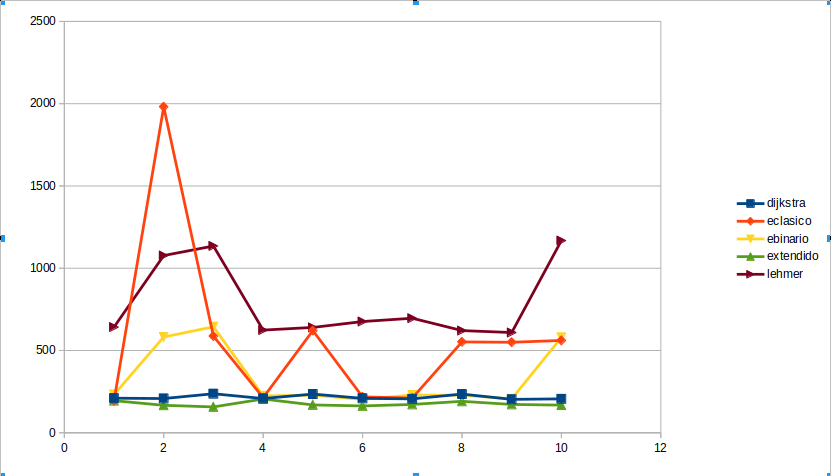
\includegraphics[scale=0.4]{./32bits.png}
 % 32bits.png: 0x0 pixel, 300dpi, 0.00x0.00 cm, bb=
 \caption{Tiempo de ejecución de 32-Bits}
 \label{fig:1}
\end{figure}



\section{Convergencia}

\begin{table}[H]
\label{tablax}
\begin{center}
\begin{tabular}{|c|c|c|c|}
\hline 
 &32b&16b&8b \\
\hline
Dijkstra& 17 & 8 & 8 \\ \hline
E. Clasico& 17& 8 & 8 \\ \hline
E. Binario& 36 & 21 & 12 \\ \hline
E. Extendido& 17 & 8 & 8 \\ \hline
Lehmer& 24 & 24 & 24 \\ \hline
\end{tabular}
\end{center}
\caption{Numero de iteraciones por algoritmos}
\end{table}

\begin{figure}[h]
 \centering
 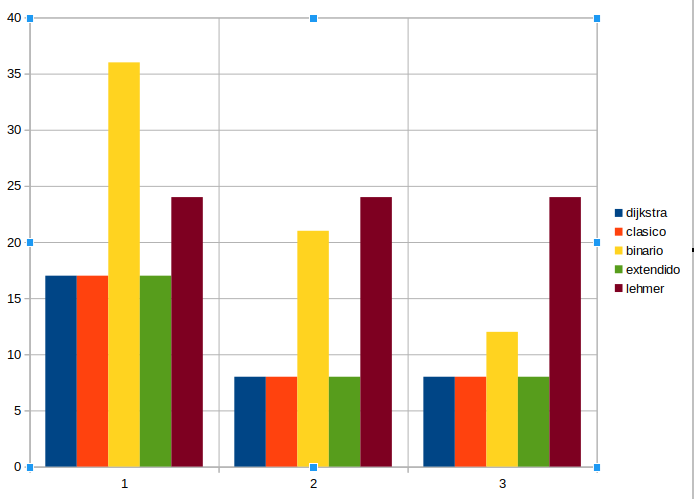
\includegraphics[scale=0.4]{./iteracion.png}
 % iteracion.png: 0x0 pixel, 300dpi, 0.00x0.00 cm, bb=
 \caption{Nro de Iteraciones en 32, 16 y 8 bits}
 \label{fig:2}
\end{figure}


\section{Acumulaci\'on de variables}

\begin{table}[H]
\label{tablax}
\begin{center}
\begin{tabular}{|c|c|c|c|}
\hline 
 &32b&16b&8b \\
\hline
Dijkstra& 50 & 50 & 50 \\ \hline
E. Clasico& 44 & 44 & 44 \\ \hline
E. Binario& 5 & 5 & 5 \\ \hline
E. Extendido& 10 & 10 & 10 \\ \hline
Lehmer& 23 & 23 & 23 \\ \hline
\end{tabular}
\end{center}
\caption{Acumulaci\'on de variables por algoritmos}
\end{table}


\begin{figure}[h]
 \centering
 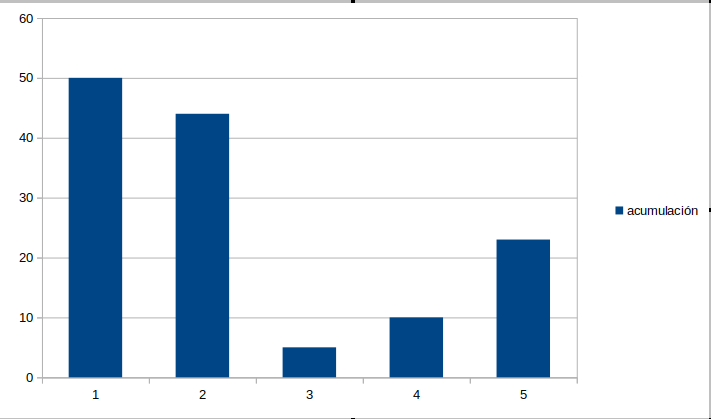
\includegraphics[scale=0.4]{./acmulac.png}
 % acmulac.png: 0x0 pixel, 300dpi, 0.00x0.00 cm, bb=
 \caption{Acumulación de variable de todos los algoritmos}
 \label{fig:3}
\end{figure}


\include{bio}
%\include{conclu}				

\appendix
%% Cap'itulos incluidos despues del comando \appendix aparecen como ap'endices
%% de la tesis.
%\include{apendiceA}
%\include{apendiceB}
%\include{apendiceC}

%% Incluir la bibliograf'ia. Mirar el archivo "biblio.bib" para m'as detales
%% y un ejemplo.
%\bibliography{biogra}
 

\end{document}
